documentclass[a4paper, amsfonts, amssymb, amsmath, reprint, showkeys, nofootinbib, twoside]{revtex4-1}
\usepackage[spanish]{babel}
\usepackage[utf8]{inputenc}
\usepackage{float}
\usepackage[colorinlistoftodos, color=green!40, prependcaption]{todonotes}
\usepackage{amsthm}
\usepackage{mathtools}
\usepackage{physics}
\usepackage{xcolor}
\usepackage{graphicx}
\usepackage[left=23mm,right=13mm,top=35mm,columnsep=15pt]{geometry} 
\usepackage{adjustbox}
\usepackage{placeins}
\usepackage[T1]{fontenc}
\usepackage{lipsum}
\usepackage{csquotes}
\usepackage[normalem]{ulem}
\useunder{\uline}{\ul}{}
\usepackage[pdftex, pdftitle={Article}, pdfauthor={Author}]{hyperref} % For hyperlinks in the PDF
%\setlength{\marginparwidth}{2.5cm}
\bibliographystyle{apsrev4-1}

\begin{document}

%El título del experimento realizado es importante.
\title{Título del experimento}


\author{Nicolás Berrío-Herrera}
\email[Correo institucional: ]{n.barbosa648@uniandes.edu.co}

%Si necesitan poner un segundo autor, deben eliminar los porcentajes (%) iniciales.
  
%\author{Second Author}
%\email{Second.Author@institution.edu}

\affiliation{Universidad de los Andes, Bogotá, Colombia.}

\date{\today} % Si lo dejan vacío no les saldrá fecha. La fecha que se muestra es del día en que se compila.

\begin{abstract}

En este se describen brevemente los objetivos y los resultados del trabajo, por lo tanto se debe dar información completa pero corta del contenido del trabajo. Se debe indicar qué fue lo que se hizo, cómo se hizo y cuáles fueron los resultados obtenidos.

\end{abstract}

\maketitle

\section{Introducción}

Se da la información básica para ubicar el problema (marco teórico) resaltando la importancia y los métodos utilizados para resolverlo. Se hace énfasis en que esta debe ser básicamente un texto corto que resuma claramente el fenómeno físico y el experimento para estudiarlo. En esta  sección se deben explicar las ecuaciones que se van a utilizar. Si existen demostraciones para dichas relaciones, se deben mostrar pasos intermedios, los pasos completos deben estar en el cuaderno.

En su mayoría, las referencias deben estar en esta sección. Se deben mencionar como: según el autor Lipari \cite{Articulo1} en su artículo \emph{Proton and neutrino extragalactic astronomy} se puede deducir que $\dots$.

También puede haber referencias las cuales se usaron pero no se parafrasearon ni se quiere hacer mención específica de la persona. \nocite{Articulo2} La segunda referencia de la bibliografía es un ejemplo de este caso. 

\section{Montaje experimental}

Descripción BREVE del método, procedimiento y montaje  experimental. Debe contener figuras, diagramas explicativos, esquema de circuitos eléctricos si aplica y las condiciones experimentales para la toma de los datos (por ejemplo entre qué valores se va a variar el voltaje en una medición). 


\begin{table*}
\caption{\label{tab:table3}Esta es una tabla amplia que ocupa toda la página con un ancho diseño de dos columnas. Se da formato con el entorno \texttt{table*}. También demuestra el uso de \textbackslash \texttt{multicolumn} en filas con entradas que abarcan
más de una columna. Las tablas deben ser de resultados obtenidos, no de datos crudos. El \emph{caption} debe tener información detallada suficiente para entender lo que se obtuvo sin tener que entrar a leer todo el documento. La tabla debe estar referenciada dentro del texto. En ocasiones se usan notas al pie adicional al \emph{caption} para resaltar detalles de datos distintos.}
\begin{ruledtabular}
\begin{tabular}{ccccc}
&\multicolumn{2}{c}{$D_{4h}^1$}&\multicolumn{2}{c}{$D_{4h}^5$}\\
Ion&1st alternative&2nd alternative&lst alternative
&2nd alternative\\ \hline
K&$(2e)+(2f)$&$(4i)$ &$(2c)+(2d)$&$(4f)$ \\
Mn&$(2g)$\footnote{The $z$ parameter of these positions is $z\sim\frac{1}{4}$.}
&$(a)+(b)+(c)+(d)$&$(4e)$&$(2a)+(2b)$\\
Cl&$(a)+(b)+(c)+(d)$&$(2g)$\footnotemark[1]
&$(4e)^{\text{a}}$\\
He&$(8r)^{\text{a}}$&$(4j)^{\text{a}}$&$(4g)^{\text{a}}$\\
Ag& &$(4k)^{\text{a}}$& &$(4h)^{\text{a}}$\\
\end{tabular}
\end{ruledtabular}
\end{table*}

\section{Resultados y análisis}

\begin{itemize}
    \item Tablas de datos: Deben estar numeradas, tituladas y rotuladas (encabezados con variables y  unidades  coherentes).  Adicionalmente  deben  estar  comentadas  o  referenciadas  en  el texto. Ver tabla \ref{tab:table3} como ejemplo. 
    \item Gráficas: Todas las gráfica deben estar numeradas, tituladas; ejes claros y de tamaño legible, escalas, variables y unidades coherentes. La mayoría de las gráficas tienen ajustes a diferentes tipos de curvas, de ser así, debe presentar en la gráfica la ecuación del ajuste realizado  con  las  variables  correspondientes  a  la  gráfica.  Todas las gráficas deben estar comentadas o referenciadas en el texto. Ver figura \ref{fig:my_label}
    
    \begin{figure}[H]
    \centering
    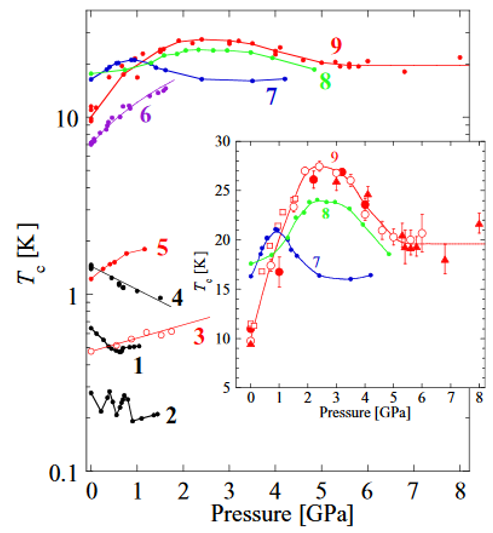
\includegraphics[scale=0.6]{GraphEj.png}
    \caption{El \emph{caption} de esta figura debe tener una descripción detallada de lo que se está mostrando como resultado. Un \emph{caption} que diga ``Gráfica de T vs P'' no dice absolutamente nada de cómo fueron obtenidos los datos y los resultados que se pueden concluir a partir de estos.}
    \label{fig:my_label}
    \end{figure}

    \item Analizar los resultados expuestos en las tablas y gráficas. Comparar estos resultados con la teoría, objetivos e hipótesis propuestas en la introducción. Se debe reportar si sus resultados y lo que aprendió en la práctica lo lleva a cumplir los objetivos propuestos, si son valores deseables o no; escriba oraciones completas que expresen sus ideas. Si se realizó ajuste, este debe estar referenciado en la gráfica y en el texto. El cálculo de la incertidumbre del resultado obtenido debe estar situado junto al resultado obtenido, no debe aparecer el resultado al inicio y la incertidumbre al final.

\end{itemize}





\section{Conclusiones}

Se deben contestar las preguntas planteadas inicialmente o dar las razones por las cuales no es posible hacerlo. Las conclusiones deben ser necesariamente una consecuencia del experimento realizado, es  decir  que  no  se  deben  tocar  aspectos  que  no  se  hayan  expuesto  en  la  sección  de resultados y análisis. Si escribe algo que no se encuentra en la sección de resultados y análisis,  esto quiere decir que hace falta incluir material en resultados y análisis. Concluir únicamente aspectos pertinentes al trabajo obtenido en el laboratorio; se deben evitar las generalizaciones que no hablan concretamente de lo que lograron o midieron en la práctica experimental. 



\bibliographystyle{abbrv}
\bibliography{Referencias}
\nocite{Ejemplo}

\section*{Apéndice de cálculo de errores}

Se deben indicar explícitamente los pasos de análisis de error que se hicieron para llegar a al(los) resultado(s). Ejemplo: la propagación de error, incertidumbre en un ajuste de mínimos cuadrados, análisis estadístico, redondeo de cifras significativas, entre otros.

Las fórmulas de cómo se obtuvieron cada uno de los valores reportados debe ser incluido como si análisis estadístico se hiciera manualmente.
\end{document}
